%% LyX 2.2.3 created this file.  For more info, see http://www.lyx.org/.
%% Do not edit unless you really know what you are doing.
\documentclass[11pt,english]{article}
\usepackage[T1]{fontenc}
\usepackage[latin9]{inputenc}
\usepackage[a4paper]{geometry}
\geometry{verbose,tmargin=3cm,bmargin=3cm,lmargin=2cm,rmargin=2cm,headheight=3cm,headsep=3cm,footskip=2cm}
\usepackage{array}
\usepackage{graphicx}

\makeatletter

%%%%%%%%%%%%%%%%%%%%%%%%%%%%%% LyX specific LaTeX commands.
%% Because html converters don't know tabularnewline
\providecommand{\tabularnewline}{\\}

\@ifundefined{date}{}{\date{}}
\makeatother

\usepackage{babel}
\begin{document}

\title{Tarea 10 de Redes}

\date{Curso 2018/2019}

\author{Jose Antonio Lorencio Abril}
\maketitle

\section*{1-}

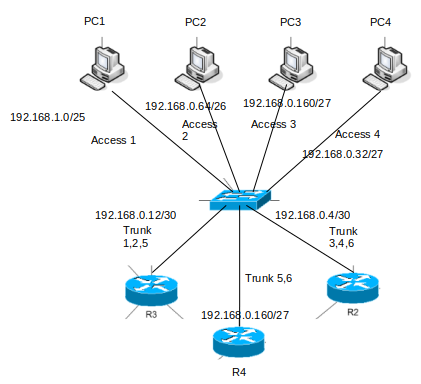
\includegraphics{pasted1}

\section*{2-}

\subsection*{a)}
\begin{flushleft}
\textbf{R1(VLAN1): }10.0.1.1/24
\par\end{flushleft}

\begin{flushleft}
\textbf{R1(VLAN2): }10.0.2.2/24
\par\end{flushleft}

\begin{flushleft}
\textbf{R2(VLAN2): }10.0.2.1/24
\par\end{flushleft}

\begin{flushleft}
\textbf{R2(VLAN3): }10.0.3.1/24
\par\end{flushleft}

\begin{flushleft}
\textbf{PC1: }10.0.1.2/24
\par\end{flushleft}

\begin{flushleft}
\textbf{PC2: }10.0.3.2/24
\par\end{flushleft}

\subsection*{b)}

\begin{tabular}{|>{\centering}p{1.5cm}|>{\centering}p{1.7cm}|>{\centering}p{1.3cm}|>{\centering}p{1cm}|>{\centering}p{1.7cm}|>{\centering}p{1.5cm}|>{\centering}p{1.7cm}|>{\centering}p{1.7cm}|>{\centering}p{1.3cm}|}
\hline 
\textbf{MAC Origen} & \textbf{MAC Destino} & \textbf{VLAN ID} & \textbf{Tipo} & \textbf{IP Origen} & \textbf{MAC Origen} & \textbf{IP Destino} & \textbf{MAC Destino} & \textbf{ICMP}\tabularnewline
\hline 
\hline 
\multicolumn{4}{|c|}{Campos Trama Ethernet} & \multicolumn{5}{c|}{Campos paquete IP/ARP/ICMP}\tabularnewline
\hline 
PC1:E0 & BCAST & 1 & ARP & 10.0.1.2 & PC1:E0 & 10.0.1.1 & 0:0 & -\tabularnewline
\hline 
R1:E0 & PC1:E0 & 1 & ARP & 10.0.1.1 & R1:E0 & 10.0.1.2 & PC1:E0 & -\tabularnewline
\hline 
PC1:E0 & R1:E0 & 1 & IP & 10.0.1.2 & - & 10.0.3.2 & - & ECHO REQ\tabularnewline
\hline 
R1:E0 & BCAST & 2 & ARP & 10.0.2.2 & R1:E0 & 10.0.2.1 & 0:0 & -\tabularnewline
\hline 
R2:E0 & R1:E0 & 2 & ARP & 10.0.2.1 & R2:E0 & 10.0.2.2 & R1:E0 & -\tabularnewline
\hline 
R1:E0 & R2:E0 & 2 & IP & 10.0.1.2 & - & 10.0.3.2 & - & ECHO REQ\tabularnewline
\hline 
R2:E0 & BCAST & 3 & ARP & 10.0.3.1 & R2:E0 & 10.0.3.2 & 0:0 & -\tabularnewline
\hline 
PC2:E0 & R2:E0 & 3 & ARP & 10.0.3.2 & PC2:E0 & 10.0.3.1 & R2:E0 & -\tabularnewline
\hline 
R2:E0 & PC2:E0 & 3 & IP & 10.0.1.2 & - & 10.0.3.2 & - & ECHO REQ\tabularnewline
\hline 
PC2:E0 & PC2:E0 & 3 & IP & 10.0.3.2 & - & 10.0.1.2 & - & ECHO REP\tabularnewline
\hline 
R2:E0 & R1:E0 & 2 & IP & 10.0.3.2 & - & 10.0.1.2 & - & ECHO REP\tabularnewline
\hline 
R1:E0 & PC1:E0 & 1 & IP & 10.0.3.2 & - & 10.0.1.2 & - & ECHO REP\tabularnewline
\hline 
\end{tabular}
\end{document}
